\documentclass{IEEEtran}
\pdfoutput=1
\usepackage{amsmath}
\usepackage{amssymb}
\usepackage{graphicx}
\usepackage{subfigure}
\usepackage{microtype}
\usepackage{cite}
\usepackage{booktabs}
\usepackage{draftwatermark}
\SetWatermarkLightness{0.85}
\usepackage{ifpdf}
\ifpdf
\usepackage{hyperref}
\fi

\title{Community Detection For Undirected Networks Using Centrality And Unsupervised Learning}
\author{Mark Ditsworth, \textellipsis}

\begin{document}
	\maketitle
	\begin{abstract}
	The computational intensity of community detection algorithms such as Louvain and spectral optimization can be prohibitive for large networks.
	Eigenvector centrality and Katz centrality are two commonly used egocentric metrics to describe the relative importance of nodes; and their calculation is also more scalable on large networks.
	In this paper, we look at the relationship between Katz centrality and eigenvector centrality, in conjunction with unsupervised machine learning, as a means of community detection.
	\end{abstract}
	
	\section{Introduction}
	In complex network analysis, community detection is often employed to find meaningful insights into the relationships between nodes. 
	Applications include customer segmentation in co-purchasing networks, subject classification in semantic networks, etc. Most popular community detection algorithms rely on iterative heuristics to attempt modularity maximization. The combinatoric nature of these algorithms make their runtime ungainly for large networks, thus requiring expensive computing power to achieve results in a reasonable amount of time.
	
	This work demonstrates the utility of Katz centrality and eigenvector centrality as features in an unsupervised machine learning algorithm to detect communities in large, undirected, weighted and unweighted networks. This method is shown to produce well-defined communities (when possible) in a much faster runtime.
	
	Sections \ref{s:mod}, \ref{s:com}, and \ref{s:cent}, detail the foundations of modularity, community detection, and Katz/eigenvector centrality, respectively. Section \ref{s:randomGraphs} demonstrates the behavior of the Katz vs. eigenvector centrality plots using ad-hoc modular networks formed from random graphs. Section \ref{s:realWorld} illustrates the utility of eigenvector and Katz centrality as features for an agglomerative clustering algorithm  that identifies prospective communities.
	 
	\section{Network Modularity}
	\label{s:mod}
	When a complex network is comprised of nodes that belong to different classes, such as community membership, it is frequently desirable to understand how interconnected they are. Are white students more likely to take classes with other white students than with students of color, or are classrooms strongly diverse? Such a question can be answered with the modularity metric.
	
	Modularity ($Q$) is calculated by (\ref{eqn:mod}), the difference between the observed fraction of edges between like nodes and the fraction expected if the edges were connected randomly \cite{Mod}.
	\begin{equation}
	\label{eqn:mod}
	Q = \frac{1}{2m}\sum_{i=1}^{n}\sum_{j=1}^{n}A_{ij}~\delta(c_i,c_j) - \frac{1}{2m}\sum_{i=1}^{n}\sum_{j=1}^{n}\frac{k_ik_j}{2m}~\delta(c_i,c_j)
	\end{equation}
	
	\noindent
	Or more simply,
	\begin{equation}
		\label{eqn:mod2}
		Q = \frac{1}{2m}\sum_{i=1}^{n}\sum_{j=1}^{n}\left(A_{ij} -\frac{k_ik_j}{2m}\right)\delta(c_i,c_j)
	\end{equation}
	
	Thus, for $Q>0$, there are more edges between like nodes than would be expected at random, indicating assortative mixing (segregation between node classes). Likewise, for $Q<0$, there are less edges between like nodes than expected, indicating disassortative mixing.
	
	While in theory, $Q$ is bounded above by 1, most network structures do not result in 0 expected edges between like nodes with randomly assigned edges. Therefore, a network with $Q$ greater than 0 signifies assortative mixing, but not necessarily the \textit{strength} of assortative mixing. For that, we must find the maximum possible value of $Q$ ($Q_{max}$) by (\ref{eqn:mod_max}).
	
	\begin{equation}
	\label{eqn:mod_max}
	Q_{max} = 1 - \frac{1}{2m}\sum_{i=1}^{n}\sum_{j=1}^{n}\frac{k_ik_j}{2m}~\delta(c_i,c_j)
	\end{equation}
	The second term is the same as that of (\ref{eqn:mod}), but the all edges are assumed to be between like nodes by setting the first term to 1. Normalizing $Q$ by $Q_{max}$ gives a more complete quantifier of the strength of assortative mixing. $Q$ may only be 0.3, but if $Q_{max}$ is only 0.34, then the network is nearly as assortatively mixed as it can be. And the normalized modularity $Q/Q_{max}=0.882$ conveys that better than $Q$ alone. 
	
	\section{Community Detection}
	\label{s:com}
	Many complex networks are not formed with predetermined class labels known for each node. It is still often useful to search for communities of nodes within the network. Most community detection algorithms assign node class such that modularity is maximized. True maximization of modularity is NP-complete \cite{NP}, so these algorithms implement iterative heuristics to guide the search.
	
	Simple modularity maximization is a popular technique for community detection\cite{simpleMM2}. It starts by randomly splitting the network into two communities. For each node, the gain in modularity caused by swapping communities is evaluated. The node whose swap results in the highest gain (or lowest reduction) is moved to the other community. This process iterates until all nodes have been moved. When a node is moved it is no longer considered in subsequent iterations. Once all nodes have been moved, the node swaps that resulted in the highest modularity are selected and made. This community grouping is used as the starting condition for the next round of the algorithm, repeating until no more gain in modularity is achieved.
	
	The most popular algorithm for community detection is arguably the Louvain method \cite{louvain}. Initially, each node is assigned to its own community. At each time step, the gain in modularity achieved by moving node $i$ to the community of each of its $j$ neighbors is calculated. Node $i$ is then placed in the community that resulted in the maximum gain in modularity. This process is repeated until no positive gain in modularity is possible.
	
	In contrast to these iterative heuristics, spectral modularity maximization attempts to optimize modularity mathematically\cite{spectral}. Recall from (\ref{eqn:mod2}) that modularity is related to the value of $A_{ij} - \frac{k_ik_j}{2m}$. The modularity matrix $\mathbf{B}$ is defined such that $B_{ij} =A_{ij} - \frac{k_ik_j}{2m}$. By numerically encoding the community labels to the set $\{0,1\}$, the Kronecker delta $\delta(i,j)$ is equivalent to $\frac{1}{2}(s_is_j + 1)$. Modularity can now be expressed by $Q = \frac{1}{4m}\mathbf{s^T}\mathbf{B}\mathbf{s}$. Relaxing the constraint that $s_i\in\{0,1\}$ to allow $s_i\in \mathbb{R}$ gives the $\max_{\mathbf{s}}Q = \mathbf{s^*}$, where $\mathbf{s^*}$ is the leading eigenvector of $\mathbf{B}$. To convert $\mathbf{s}$ back to the domain $\{0,1\}$, the sign function is employed.
	
	Each of the above community detection algorithms requires either numerous iterations through combinatorial partitions of the network nodes, or linear algebraic operations on the adjacency matrix. More recent literature on community detection extends the use of these methods, altering calculations and processes, but do not deviate from the iterative maximization of modularity\cite{Leider,alpha}. For large complex networks, the computational and memory expense may prove impractical. The iterative calculation of Katz and eigenvector centrality are much more scalable on large networks. And as we will show, for network communities of sufficient modularity and difference in density, the plot of Katz centrality versus eigenvector centrality (hereafter referred to as the Katz-eigen plot) can reveal clusters of nodes that indicate community membership. Figure \ref{fig:example} illustrates two such cases.
	
	\section{Eigenvector and Katz Centrality}
	\label{s:cent}
	The eigenvector centrality of node $i$ is measured by the scaled sum of the eigenvector centralities of it's neighbors (in-neighbors in the case of directed networks) as shown in (1), where $\lambda_1$ is the leading eigenvalue of the adjacency matrix $\mathbf{A}$ \cite{EVC}.
	\begin{equation}
	\label{eqn:evc}
	x_i = \frac{1}{\lambda_1}\sum_{j=1}^{n}A_{i,j}~x_j
	\end{equation}
	Since the centralities are interdependent, this is calculated iteratively until the centralities reach a steady-state. Once in steady-state, the matrix representation of (\ref{eqn:evc}) can be written by (\ref{eqn:evc_m}).
	\begin{equation}
	\label{eqn:evc_m}
	\mathbf{x} = \frac{1}{\lambda_1}A\mathbf{x}
	\end{equation}
	This is just the equation for the eigenvector of $\mathbf{A}$ corresponding to the eigenvalue $\lambda_1$, hence the name eigenvector centrality.
	
	Katz centrality is calculated similarly to eigenvector centrality, but with free centrality $\beta$ given to all nodes, as shown in (\ref{eqn:katz})\cite{katz}. The matrix representation is shown in (\ref{eqn:katz_m}).
	\begin{equation}
	\label{eqn:katz}
	x_i = \alpha\sum_{j=1}^{n}A_{i,j}~x_j + \beta
	\end{equation}
	\begin{equation}
	\label{eqn:katz_m}
	\mathbf{x} = (I-\alpha A)^{-1}~\beta
	\end{equation}
	If $\alpha$ is 0, all nodes' centralities are $\beta$. If $\alpha$ is $\frac{1}{\lambda_1}$, $(I-\alpha A)$ is singular, the inverse is undefined and the centralities diverge to infinity. For $0 < \alpha < \frac{1}{\lambda_1}$, the centralities converge. This centrality measure was created to account for the fact that in directed networks without strongly connected components, there are no nodes with non-zero eigenvector centrality. The free centrality guarantees all nodes have at least some centrality.
	
	It is evident from (\ref{eqn:evc}) and (\ref{eqn:katz}) that generally speaking, a node's Katz centrality is greater than it's eigenvector centrality. Normally, the exact value of a node's centrality is not so important as its relative value, so as to discern the order of importance. But the amount by which Katz centrality is greater than eigenvector centrality can serve as in important indicator, as well will see, for differences in local connectivity.
	
	\section{Application to Ad-hoc Modular Networks}
	\label{s:randomGraphs}
	We demonstrate the utility of the Katz-eigen plot first on synthetic, ad-hoc modular networks. These networks are constructed to guarantee the existence of two communities, but with modularity and relative density more or less controllable. 
	
	\begin{figure}
		\centering
		\subfigure[][]{
			\label{fig:example-a}
			\includegraphics[width=0.98\linewidth]{../BA_Graph/example.png}}
		\subfigure[][]{
			\label{fig:example-b}
			\includegraphics[width=0.98\linewidth]{../ER_Graph/example.png}}
		\caption{Katz vs eigenvector centrality plots for the two predetermined communities using random graphs. $n_1=n_2=250$ and $\mu=800$. \subref{fig:example-a} used the BA model with each node adding 20 edges for green community and 10 edges for the blue. \subref{fig:example-b} used the ER model with $p=0.1$ for both communities. In each figure, the black lines are the linear trend-lines for each community.}
		\label{fig:example}
	\end{figure}

	\begin{figure}
		\centering
		\subfigure[][]{
			\label{fig:angle-a}
			\includegraphics[width=0.98\linewidth]{../BA_Graph/angle.png}}
		\subfigure[][]{
			\label{fig:angle-b}
			\includegraphics[width=0.98\linewidth]{../ER_Graph/angle.png}}
		\caption{Plot of the average angle between the two clusters in the Katz-eigen plot over 20 ad-hoc modular networks. The angle is calculated by finding the difference in arctangent of the linear slope of each cluster. \subref{fig:example-a} uses the BA model for network generation. \subref{fig:example-b} uses the ER model. In both cases, $n_1=n_2=250$ remains constant.}
		\label{fig:angle}
	\end{figure}
	
	\begin{figure}
		\centering
		\subfigure[][]{
			\label{fig:dist-a}
			\includegraphics[width=0.98\linewidth]{../BA_Graph/cluster_distance.png}}
		\subfigure[][]{
			\label{fig:dist-b}
			\includegraphics[width=0.98\linewidth]{../ER_Graph/cluster_distance.png}}
		\caption{Plot of the average distance between the two clusters in the Katz-eigen plot over 20 ad-hoc modular networks. The distance is defined as the euclidean distance between the centroids of the lower half of the cluster. This definition causes the distance to be measured closer to the base of each cluster. \subref{fig:example-a} uses the BA model for network generation. \subref{fig:example-b} uses the ER model. In both cases, $n_1=n_2=250$ remains constant.}
		\label{fig:dist}
	\end{figure}
	
	%\section{Application to Ad-hoc Modular Networks}
	%\label{s:randomGraphs}
	%We demonstrate the utility of the Katz-eigen plot first on synthetic, ad-hoc modular networks. These networks are constructed to guarantee the existence of two communities, but with modularity and relative density more or less controllable. 
	
	The ad-hoc modular networks are formed as follows. Two random graphs are generated (in this work we use the exponential-random (ER) model\cite{ER} and the Barab\'asi-Albert (BA) model\cite{BA}) with $n_1$ and $n_2$ nodes. 
	Adjusting the $p$ parameter (the probability of edge existance) for the ER model and the $m$ parameter (the number of edges added by each new node) for the BA model controls the density of each random network.
	
	The two networks are then joined by adding $\mu$ edges between randomly (uniformly) selected nodes from each, thereby creating one network of two communities. Increasing $\mu$ decreases the modularity of the network and vice versa.
	
	Figure \ref{fig:example} shows the plot of the normalized Katz vs eigenvector centrality on ad-hoc modular networks. When calculating Katz centrality, $\alpha$ and $\beta$ are se to 0.001 and 1, respectively. In order to allow for comparison across different networks, Katz and eigenvector centralities will be normalized to be between $[0,1]$.
	
	The green community is created to be more dense than the blue, and there are clear differences in the Katz-eigen plot. A linear regression of each community shows differing slope, and there is a shift in the lowest eigenvector and Katz centrality of each community.
	
	Performing parameter sweeps of $p$ or $m$ and  of $\mu$ allows for the characterization of the Katz-eigen plot across varying modularities and differences in average local clustering coefficient between the communities.
	A node's local clustering coefficient (LCC) is the fraction of pairs of its neighbors that are themselves neighbors.
	When the ad-hoc networks are created, the average LCC of each subnetwork is calculated before they are joined. Figures \ref{fig:angle} - \ref{fig:length} refer to the average LCC ratio. This is the ratio for the average LCC of the blue community to that of the green community. As this ratio gets closer to 1, it is understood that the relative density of each community becomes more similar.
	
	Figure \ref{fig:angle} shows that the angle $\theta$ between the clusters  increases with modularity. Higher assortative mixing in the network is associated with more separability in the Katz-eigen plot. As the relative densities of the communities approach equivalency, $\theta$ becomes more sensitive to modularity. A near-linear relationship at lower average LCC ratios turns more quadratic at higher LCC ratios. At low average LCC ratios and high modularity, the blue cluster on the Katz-eigen plot is condensed into more of a blob, causing linear regression to perform erratically This causes the chaotic behavior seen at high modularity and low average LCC ratio.
	
	In addition to $\theta$ changing with modularity and average LCC ratio, the euclidean distance between the bases of the green and blue clusters changes as well. Figure \ref{fig:dist} shows the cluster distance increasing with stronger assortative mixing and decreasing with higher average LCC ratio. Again, we see the higher sensitivity to modularity when the average LCC ratio approaches 1.
	
	The relative size of the green and blue clusters is also dependent on modularity and density. Figure \ref{fig:length} shows the cluster length ratio between the green and blue communities. As assortative mixing increases, the green cluster increases in length compared to the blue cluster. The closer the communities' densities are to each other, the more assortative mixing required to reach a given length ratio.
	
	That differences in community density, connectivity, and modularity result in discernible differences in the Katz-eigen plot suggests that this plot can be useful for community detection in networks. Similar outcomes for ad-hoc networks constructed with the ER and BA models indicate that networks with exponential or scale-free degree distributions are both apt to demonstrate this phenomenon.

	\begin{figure}
		\centering
		\subfigure[][]{
			\label{fig:length-a}
			\includegraphics[width=0.98\linewidth]{../BA_Graph/cluster_length.png}}
		\subfigure[][]{
			\label{fig:length-b}
			\includegraphics[width=0.98\linewidth]{../ER_Graph/cluster_length.png}}
		\caption{Plot of the average ratio of cluster length in the Katz-eigen plot over 20 ad-hoc modular networks. Cluster length is defined as the length of the diagonal of the smallest rectangle that encapsulates all points of the cluster. \subref{fig:example-a} uses the BA model for network generation. \subref{fig:example-b} uses the ER model. In both cases, $n_1=n_2=250$ remains constant.}
		\label{fig:length}
	\end{figure}

	\begin{figure}
	\centering
	\includegraphics[width=0.98\linewidth]{dblp_2_kev.png}
	\caption{Katz-eigen plot of the sampled DBLP network. For Katz centrality, $\alpha = 1e-4$ and $\beta = 1$.}
	\label{fig:dblp_pre}
	\end{figure}

	\begin{figure}
	\centering
	\includegraphics[width=0.98\linewidth]{dblp_cluster.png}
	\caption{Katz-eigen plot of the sampled DBLP clustering showing the clusters found by agglomerative clustering algorithm. The affinity measurement is cosine similarity.}
	\label{fig:dblp_cluster}
	\end{figure}

	\section{Performance on Real World Networks}
	\label{s:realWorld}
	To further test this proposed community detection method we look at real-world networks. Networks with predetermined ``ground-truth" communities are especially of interest since they can provide a measurable benchmark. However, it should be noted that the existence of ``ground-truth" communities may not translate to a strong assortatively mixed network. For example, in a network of United States congressional seats based on vote-sharing, we can define ``ground-truth" communities by gender or age. But the modularity due to these communities will not out-perform that caused by communities of political party \cite{congress}.
	
	One network with predetermined ``ground-truth communities" is the DBLP network\cite{DBLP} obtained from the Stanford Network Analysis Project\cite{SNAP}. The DBLP is a co-authorship network of computer science publications. ``Publication venue, e.g, journal or conference, defines an individual ground-truth community; authors who published to a certain journal or conference form a community."
	
	There are 317,080 nodes in over 5,000 ``ground truth" communities in this network. We sample the nodes in the two largest communities and take the induced subgraph, leaving our network with 13,326 nodes. Since communities are defined from publication venue, it is possible for nodes to belong to multiple communities. The Katz-eigen plot is shown in Figure \ref{fig:dblp_pre}. The orange and blue dots represent the nodes in communities one and two, respectively, and the green dots are nodes that are in both.
	
	\begin{figure}
		\centering
		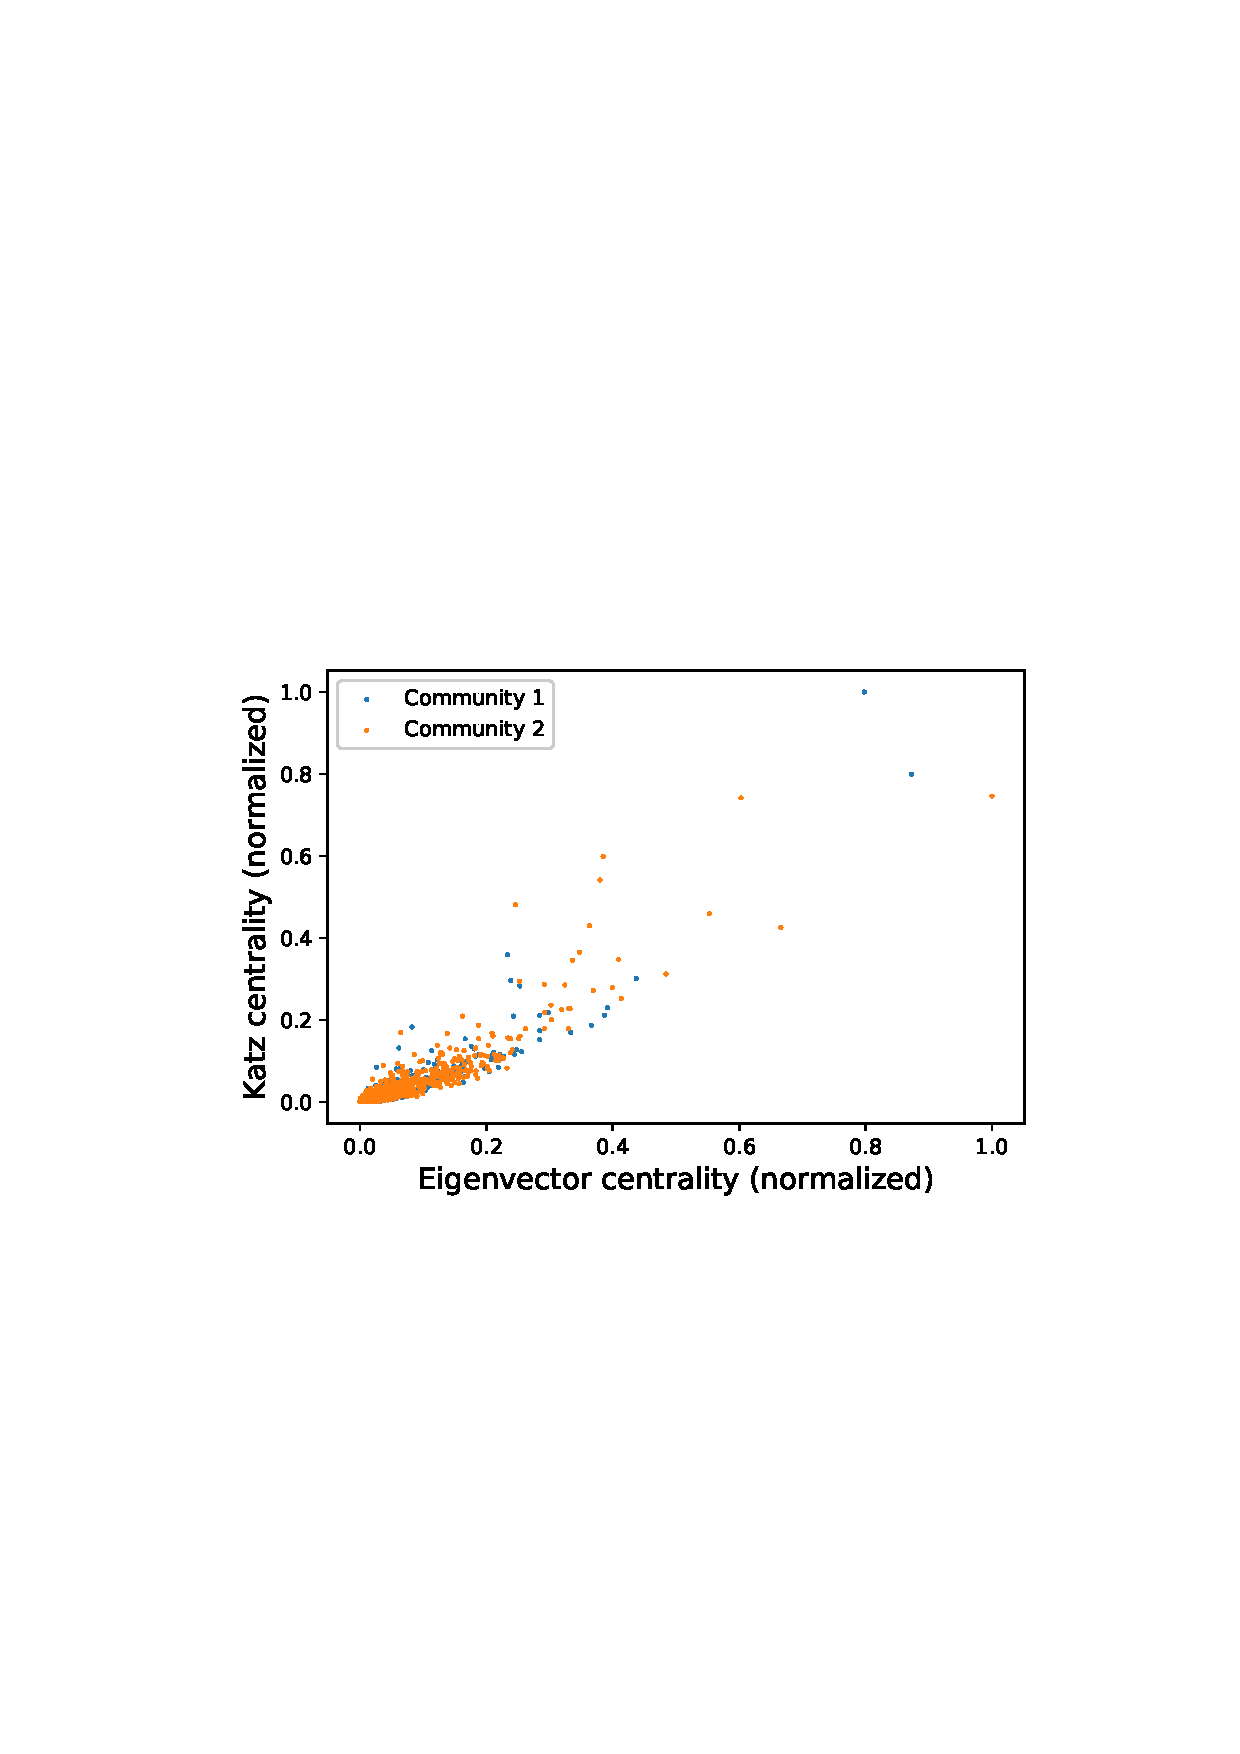
\includegraphics[width=0.98\linewidth]{youtube.png}
		\caption{Katz-eigen plot of two largest communities in the YouTube friendship network. This sampled graph has 3,269 nodes, and 25\% of nodes are members of both communities. %The lack of distinct clusters corresponds to poor modularity in the network.
		}
		\label{fig:youtube}
	\end{figure}
	
	\begin{figure}
		\centering
		\includegraphics[width=0.98\linewidth]{amazon_product.png}
		\caption{Katz-eigen plot of the two largest communities in the Amazon product network. The sampled graph has 328 nodes, with all nodes belonging to both ``ground-truth" communities. The red, blue, and green clusters are identified with agglomerative clustering using cosine affinity.}
		\label{fig:amazon_product}
	\end{figure}
	
	\begin{figure}
		\centering
		\includegraphics[width=0.98\linewidth]{amazon_health_clustered.png}
		\caption{The Katz-eigen plot of the Amazon health product review network. The red and blue clusters are identified with the agglomerative clustering algorithm, using cosine affinity.}
		\label{fig:amazon_health}
	\end{figure}
	
	\begin{figure}
		\centering
		\includegraphics[width=0.98\linewidth]{amazon_beauty_clustered.png}
		\caption{The Katz-eigen plot of the Amazon beauty product review network. The red, blue, and green clusters are identified with the agglomerative clustering algorithm, using cosine affinity.}
		\label{fig:amazon_beauty}
	\end{figure}
	
	We see two distinct vectors in the Katz-eigen plot: one dominated by primarily blue nodes, and the other dominated by orange and green. The wide angle between them suggests high modularity. In fact, between the two distinct communities, $Q=0.438$, and $Q/Q_{max} = 0.827$.
	
	Assume that these labels were not provided before hand. Using agglomerative clustering (implemented with Scikit-learn \cite{scikit-learn}) with complete linkage and cosine similarity as the affinity measurement, we can define two clusters of nodes based on proximity to the two prominent vectors in the Katz-eigen plot. The results of this clustering is shown in Figure \ref{fig:dblp_cluster}. Assuming these two node groupings, $Q=0.022$ and $Q/Q_{max}=0.565$. The strength of assortative mixing is 70\% of that seen with the ``ground-truth" community labels. $Q$ is so low here due to the imbalance in cluster size. The orange cluster consists of only 533 nodes, whereas the blue cluster contains the remaining 12,793 nodes. Thus, only a small fraction of the edges can be contained in the orange cluster.
	
	As suggested by the trends in Section \ref{s:randomGraphs}, lack of modular communities results in little-to-no distinguishable clusters in the Katz-eigen plot. This is illustrated in a YouTube friendship network, where ``ground-truth" communities are defined by user groups \cite{DBLP,youtube}. The Katz-eigen plot of this network is shown in Figure \ref{fig:youtube}. The significant overlap of the two communities on the plot indicates low modularity: $Q=0.049$ and $Q/Q_{max}=0.109$. In this case, the ``ground-truth" communities do not reflect the properties of communities from a networks perspective.
	
	Similarly, two largest ``ground-truth" communities in the Amazon product network \cite{youtube,DBLP} contain the same nodes. As a result, $Q=0$ and the Katz-eigen plot of the two communities are completely overlapped. These two defined communities provide no utility to understanding the network. But, as depicted in Figure \ref{fig:amazon_product}, there are three clusters of nodes identified by agglomerative clustering. Using these communities, $Q=0.254$ and $Q/Q_{max}=0.659$, this provides more insight into groupings within the network compared to the ``ground-truth" communities.
	
	%Note that in Figures \ref{fig:dblp_pre} and \ref{fig:dblp_cluster} that the lower vector is positioned much closer than the $x$ axis than we see in the ad-hoc networks. The position of the green cluster vector in Figure \ref{fig:example} remains relatively consistent with the $[1,1]$ vector throughout different ad-hoc networks; the blue cluster's vector moves more dramatically. This indicates that, when normalized, a node in the green community Katz centrality is roughly equivalent to its eigenvector centrality. Whereas a node in the blue community significantly benefits from the free centrality provided by Katz.
	
	%Comparatively, in Figures \ref{fig:dblp_pre} and \ref{fig:dblp_cluster} we have one community who's centrality is helped by free Katz centrality, and another who's is harmed. Wait, no, this has to do with which community has the node with the highest Katz centrality \textellipsis
	
	%We now look at a real world network that happens to demonstrate the $[1,1]$ vector trend, and the Katz-eigen method works well on community detection.
	
	Many, if not most, networks do not contain ``ground truth" communities, hence the need for community detection algorithms. We now show the applicability of the Katz-eigen community detection method to other real-world networks without ``ground-truth" communities, and judge its effectiveness solely by the normalized modularity achieved from the detected communities.
	
	We sample the 5-core dataset of Amazon health product reviews\cite{amazon} from January to July of 2014. A review network is constructed where nodes (user accounts) are connected with weighted edges representing the number of common products reviewed. The resulting network has 25,026 nodes. Figure \ref{fig:amazon_health} shows the Katz-eigen plot of this network after applying the agglomerative clustering algorithm to identify communities. With the red and blue assigned communities, modularity is quite high: $Q=0.393$ and $Q/Q_{max}=0.808$. There are no ``ground-truth" communities given for this network, but the high normalized modularity indicates good detection of communities.
	
	Clustering by cosine affinity on the Katz-eigen plot has shown the ability to detect more than two communities. Figure \ref{fig:amazon_beauty} shows the Katz-eigen plot of another Amazon review network of beauty products (created the same way as the health product network). Here, there are three clear clusters, indicating three communities in the 13,043 node network. With these defined communities, $Q=0.268$ and $Q/Q_{max}=0.721$.
	
	
	\section{Conclusions}
	\label{s:conc}
	In this work, we have showed that Katz and eigenvector centrality can serve as features for community detection. For undirected networks with sufficient modularity and/or difference in density of it's communities, the Katz-eigen plot displays clusters centered around distinct vectors. Agglomerative clustering with cosine similarity can identify these clusters, thereby allowing for automated identification of community membership for many nodes. A summary of this method's performance is given in Figure \ref{tab:performance}.
	
	This method was shown to detect communities with comparable modularity to that of pre-labeled ``ground truth" communities in real world networks. In other real world networks without node labels, the communities detected by the Katz-eigen method were strongly assortatively mixed, suggesting well-performing community detection.
	
	Future research will investigate the Katz-eigen community detection method on directed networks. Furthermore, the impact of edge weights on this method should be more closely understood, particularly for signed networks.
	
	All code for this project is available at (link to github).
	
	\begin{figure}
		\centering
		\begin{tabular}{lcc}
			\toprule
			\textbf{Network} & \textbf{Ground-truth} $Q/Q_{max}$ & \textbf{Detected $Q/Q_{max}$}\\
			\midrule
			DBLP & 0.827 & 0.565\\
			YouTube & 0.109 & N/A\\
			AMZN Product & 0.000 & 0.659\\
			AMZN Health & N/A & 0.808\\
			AMZN Beauty & N/A & 0.721\\
			\bottomrule
		\end{tabular}
		\caption{Summary of the performance of Katz-eigen community detection on real-world networks.}
		\label{tab:performance}
	\end{figure}
	
	\section*{Acknowledgements}
	Thank you to \textellipsis
	%Dr. Justin Ruths with the Department of Systems Engineering at the University of Texas at Dallas.

	\bibliography{references}
	\bibliographystyle{IEEEtran}
\end{document}